\documentclass[t]{beamer}

%\documentclass[handout, t]{beamer}
\setbeamertemplate{navigation symbols}{}
\usepackage{pstricks}
\usepackage{mathtools}
\usepackage{amsfonts}
\usepackage{mathrsfs}
\usepackage{amsmath}
\usepackage{physics}
\setbeamertemplate{navigation symbols}{}
\usepackage{bm}
\usepackage[UTF8]{ctex}
\usetheme{AnnArbor}
\usefonttheme{serif}
\useinnertheme{rounded}
\usecolortheme{beaver}
\setbeamertemplate{blocks}[rounded][shadow=true]

\newcommand{\dif}{{\;\rm d}}
\usepackage{graphicx}
\usepackage{pgf}
\usepackage{tikz}
\usetikzlibrary{arrows, decorations.pathmorphing, backgrounds, positioning, fit, petri, automata}
\tikzset{>=stealth}

\usepackage{setspace}
\setmainfont{Times New Roman}
\setCJKmainfont{Microsoft YaHei}
% \setCJKmainfont{苹方}   % 使用苹果MAC系统,请使用这个选项,并将上面的命令用%注释掉

\hypersetup{pdfpagemode=FullScreen}
\renewcommand{\Pr}{\mathbb{P}}
\usepackage{blkarray}


\setbeamercolor{block title}{bg=red!10!white}
\setbeamercolor{block body}{bg=gray!10!white}

\usepackage{multicol}
\newcommand{\E}{\mathbb{E}}
\newcommand{\EP}{\mathbb{E}^{\mathbb{P}}}
\newcommand{\EQ}{\mathbb{E}^{\mathbb{Q}}}
\newcommand{\Var}{{\rm Var}}
\newcommand{\Cov}{{\rm Cov}}


\begin{document}
\fontsize{11}{18}\selectfont


\CTEXindent

\title{第五章~~随机微分方程概论}
\author{金融数学}
\date{
	中国人民大学出版社}
\begin{frame}
	\maketitle
\end{frame}

\begin{frame}{随机微分方程(Stochastic Differential Equation, SDE)}
通过对SDE的求解,我们可以更深刻地认识随机过程的演化规律。

随机微分方程是微分方程的扩展。随机过程函数本身的导数不可定义,所以一般解微分方程的概念不适用于随机微分方程。

随机微分方程多用于对一些多样化现象进行建模,比如不停变动的股票价格,部分物理现象如热扰动等。
\end{frame}

\begin{frame}{本章内容}
\tableofcontents

\end{frame}


\section{引言}


\begin{frame}{SDE的例子:几何布朗运动}
\[\dif S(t)=\mu S(t)\dif t+\sigma S(t) \dif W(t)\]
其中:$S(t)$是随机过程;$\mu$和$\sigma$均是常数;$W(t)$是标准布朗运动。该方程在金融领域可以用来刻画股票等金融资产的价格演化。

SDE有无穷多个可能的解,为了对解加以限定,需要加入初值条件(initial value condition),比如:$S(0)=S_0$。
\end{frame}

\begin{frame}{普通微分方程$\dif S(t)=\mu S(t)\dif t,\quad S(0)=S$}
求解思路:
\begin{enumerate}
\item 采用分离变量法(separation of variables),将公式右侧的$S(t)$提到左侧,即:
\[\frac{\dif S(t)}{S(t)}=\mu \dif t \]
\item 对公式两侧取积分,可得:
\[\int^t_0\frac{\dif S(u)}{S(u)}=\int^t_0\mu \dif u \quad \Rightarrow\quad \ln S(t)-\ln S(0)=\mu t \]
\item 将初值条件代入,最终可得:
\[S(t)=S(0)e^{\mu t}= S\cdot e^{\mu t}\]
\end{enumerate}
\end{frame}

\begin{frame}{几何布朗运动SDE的求解}
布朗运动$W(t)$是处处连续且处处不可微的,这一特征造成了我们不能使用通常求解微分方程的相关方法对SDE进行分析和求解。
\[\begin{split}
\frac{\dif S(t)}{S(t)}=\mu \dif t &\quad\Rightarrow\quad \dif \ln[S(t)]=\mu \dif t\\
\frac{\dif S(t)}{S(t)}=\mu \dif t+\sigma \dif W(t) &\quad\not\Rightarrow\quad \dif \ln[S(t)]=\mu \dif t+\sigma \dif W(t)
\end{split} \]

\begin{block}{注意:}
上式的原因在于布朗运动$W(t)$的二次变差不为零,我们需要使用伊藤引理进行求解。
\end{block}
\end{frame}

\begin{frame}{几何布朗运动SDE的求解(cont.)}
假设$f(x)=\ln(x)$,根据伊藤引理可得:
\begin{equation*}
\begin{split}
\dif f(S(t))&=f_t\dif t+f_S\dif S+\frac{1}{2}f_{SS}[\dif S]^2\\
&=0+\frac{1}{S}[\mu S\dif t+\sigma S \dif W]+\frac{1}{2}\left(-\frac{1}{S^2}\right)\sigma^2S^2\dif t\\
&=\mu \dif t+\sigma \dif W\;{\color{red}-\frac{1}{2}\sigma^2\dif t}\\
\end{split}
\end{equation*}
因此:
\begin{equation*}
\dif \ln S(t)=\left(\mu\;{\color{red}-\frac{1}{2}\sigma^2} \right) \dif t+\sigma\dif W(t)
\end{equation*}
在此基础上,我们实现了类似于微分方程中的分离变量方法。接下来对上式两端取积分。
\end{frame}

\begin{frame}{几何布朗运动SDE的求解(cont.)}\normalsize
\begin{equation*}
\dif \ln S(t)=\left(\mu -\frac{1}{2}\sigma^2  \right) \dif t+\sigma\dif W(t)
\end{equation*}
上式两端取积分可得:
\begin{align*}
\int^t_0\dif \ln S(u)&=\int^t_0\left(\mu-\frac{1}{2}\sigma^2 \right) \dif u+\int^t_0\sigma\dif W(u) \\
\ln S(t)-{\color{blue}\ln S(0)}&=\left(\mu-\frac{1}{2}\sigma^2 \right)t+ \sigma [W(t)-W(0)]\\
\ln S(t)&={\color{blue}\ln S_0}+\left(\mu-\frac{1}{2}\sigma^2 \right)t+ \sigma W(t)
\end{align*} 
最终得到:
\begin{equation*}
S(t)=S_0\cdot \exp\left[\left(\mu-\frac{1}{2}\sigma^2 \right)t+ \sigma W(t)\right]
\end{equation*}


\end{frame}

\begin{frame}{几何布朗运动SDE的解}
几何布朗运动SDE
\[\begin{cases}
\dif S(t)=\mu S(t)\dif t+\sigma S(t) \dif W(t)\\
S(0)=S_0
\end{cases}\]
解如下:
\begin{equation*}
S(t)=S_0\cdot \exp\left[\left(\mu-\frac{1}{2}\sigma^2 \right)t+ \sigma W(t)\right]
\end{equation*}
相应的,
\[\ln S(t)\sim \mathcal{N}\left(\ln S_0+\left[\mu-\frac{1}{2}\sigma^2 \right]t, \sigma^2 t\right)  \]
因此,$\ln S(t)$服从正态分布。对应的$S(t)$则是服从对数正态分布(log-normal distribution)。
\end{frame}

\begin{frame}{对数正态分布的概率密度函数图}
	\centering
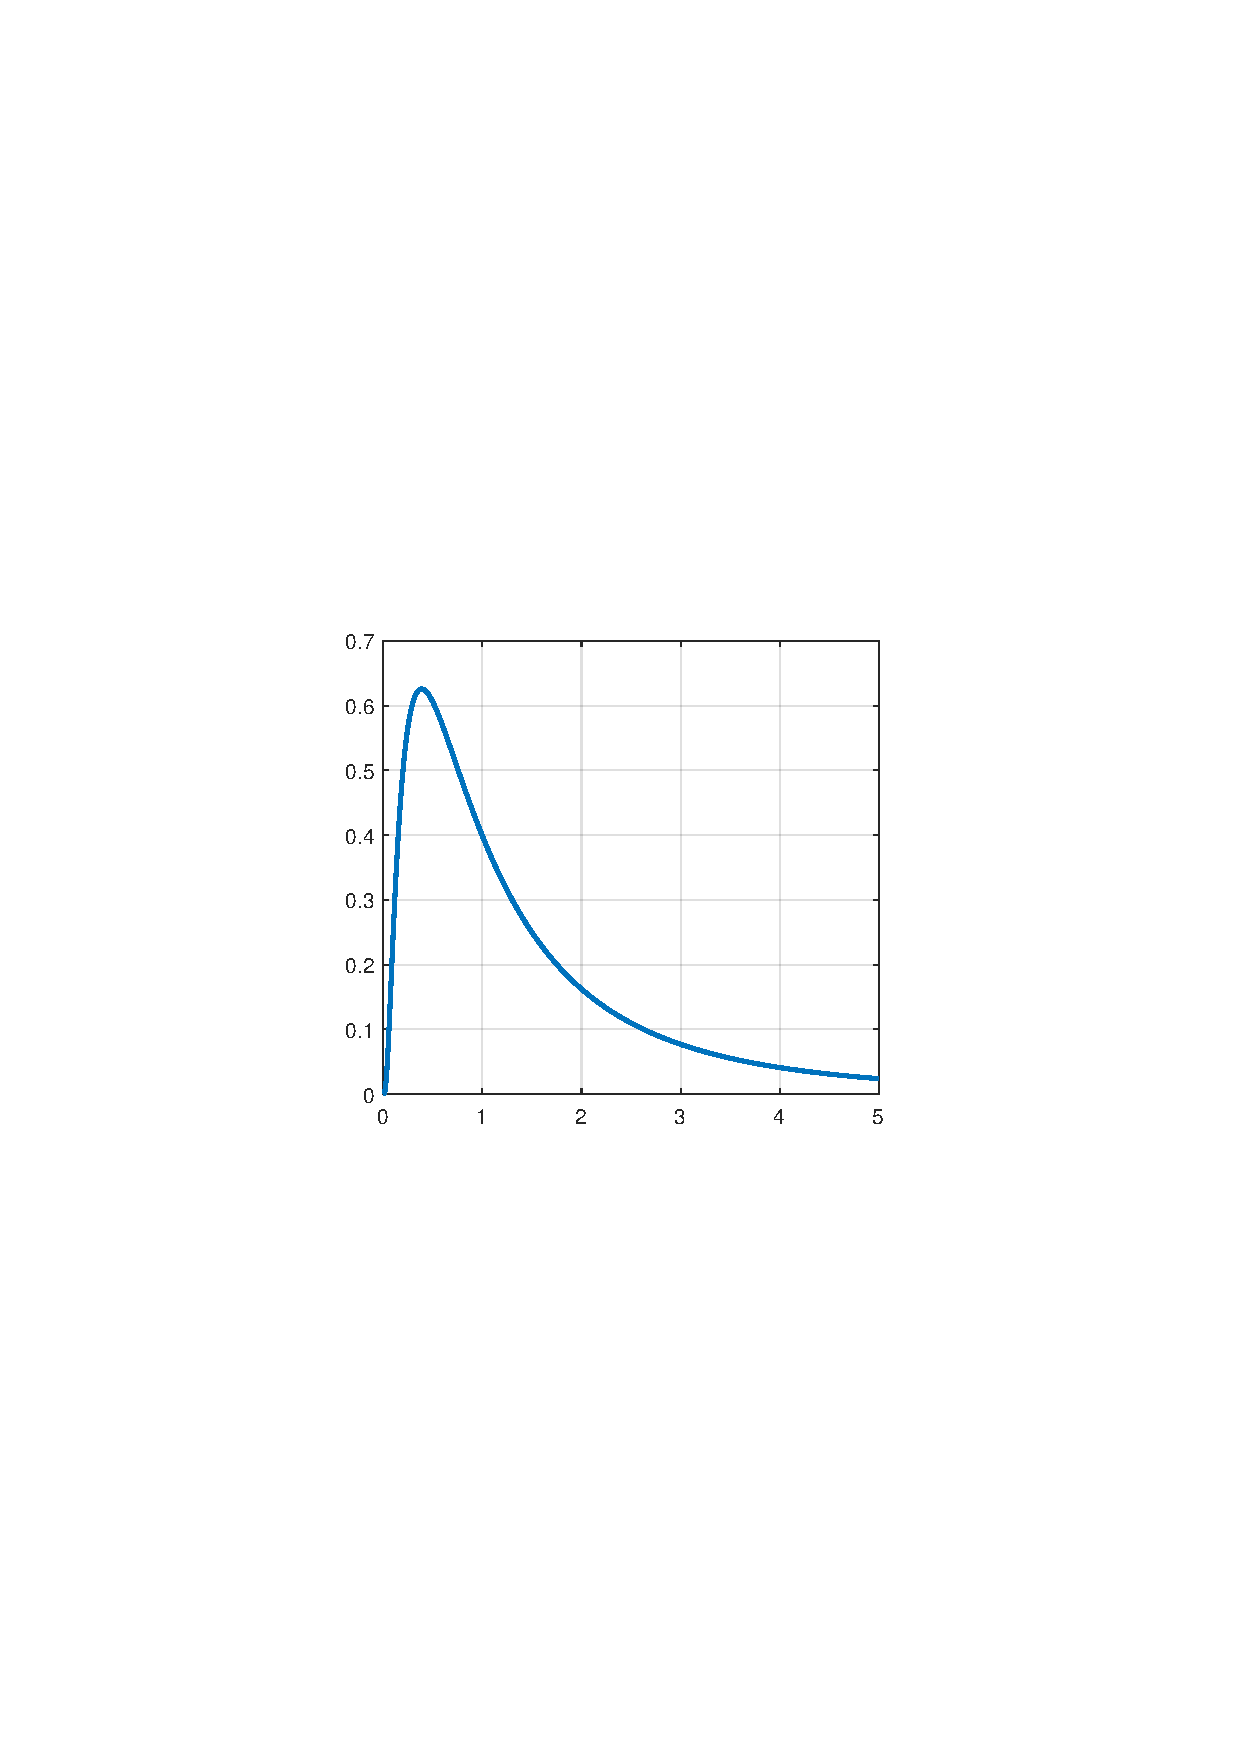
\includegraphics[scale=.8]{fig/lognormal.pdf}
\end{frame}

\begin{frame}{$S(t)$期望和方差}
服从对数正态分布的$S(t)$期望和方差分别如下:
\[\begin{split}
\E[S(t)]&=\exp\left[\ln S_0+\mu t \right]=S_0\cdot e^{\mu t}\\
\Var[S(t)]&=\exp\left[2\ln S_0+2\mu t \right]\left[\exp(\sigma^2 t)-1\right]=S^2_0 e^{2\mu t}\cdot \left(e^{\sigma^2 t}-1\right) 
\end{split} \]

\begin{block}{说明:}
本章只涉及线性随机微分方程的求解问题。
\end{block}
\end{frame}

\section{线性随机微分方程的分类}
\begin{frame}{一维线性SDE的基本形式}
\begin{equation*}
\dif X(t)=\alpha \big(t,X(t)\big)\dif t+\beta\big(t,X(t)\big)\dif W(t)
\end{equation*}
其中:$$\alpha \big(t,X(t)\big)=a_1(t)X(t)+a_2(t),\quad \beta \big(t,X(t)\big)=b_1(t)X(t)+b_2(t)$$

$\alpha \big(t,X(t)\big)$称作漂移项(drift term);$\beta \big(t,X(t)\big)$称为扩散项(diffusion term)。另外SDE还有一个相应的初值条件(initial value condition),比如:$X(0)=X_0$。
\end{frame}

\begin{frame}{线性SDE的分类}
对于一维线性SDE:
\[\dif X(t)=\bigg[a_1(t)X(t)+a_2(t)\bigg]\dif t+\bigg[b_1(t)X(t)+b_2(t)\bigg]\dif W(t)\]

\begin{enumerate}
\item 若所有的系数($a_1,a_2,b_1,b_2$)均是常数,则称为自治(autonomous)线性SDE,即系数不是时变的;
\item 若$a_2=b_2=0$,则称为齐次(homogeneous)线性SDE;
\item 若$b_1=0$,则线性SDE具有加性噪声(additive noise);
\item 若$b_2=0$,则线性SDE具有乘性噪声(multiplicative noise)。
\end{enumerate}
\end{frame}

\begin{frame}{举例1:几何布朗运动}
股票价格$S(t)$服从几何布朗运动如下:
\[\dif S(t)=\mu S(t)\dif t+\sigma S(t) \dif W(t) \]
其中:$\mu$和$\sigma$均是常数,通过比对可以看出:
\[a_1=\mu,\quad a_2=0,\quad b_1=\sigma,\quad b_2=0 \]
因此,用来刻画股价变动的几何布朗运动属于自治线性SDE,并且具有乘性噪声。
\end{frame}

\begin{frame}{举例2:瓦西切克(Vasicek)模型}
刻画利率$r(t)$变动的瓦西切克模型如下:
\[\dif r(t)=\big(\alpha-\beta r(t)\big)\dif t+\sigma \dif W(t) \]
其中:$\alpha,\;\beta,\;\sigma$均是大于零的常数,通过比对可以看出:
\[a_1=-\beta,\quad a_2=\alpha,\quad b_1=0,\quad b_2=\sigma \]
因此,用来刻画短期利率变动的瓦西切克模型属于自治线性SDE,并且具有加性噪声。该模型来自于奥伦斯坦-乌伦贝克过程(Ornstein-Uhlenbeck process),简称O-U过程,并且该过程具有均值回复的特征。

\end{frame}


\begin{frame}{举例3:赫尔-怀特(Hull-White)模型}
刻画利率$r(t)$变动的赫尔-怀特模型如下:
\[\dif r(t)=\big(\alpha(t)-\beta(t) r(t)\big)\dif t+\sigma(t) \dif W(t)  \]
其中:$\alpha(t),\;\beta(t),\;\sigma(t)$均是均值大于零的函数,通过比对可以看出:
\[a_1=-\beta(t),\quad a_2=\alpha(t),\quad b_1=0,\quad b_2=\sigma(t) \]
因此,赫尔-怀特模型属于具有加性噪声的线性SDE。对比瓦西切克模型,此处的模型仍然具有均值回复的特征,只是相应的系数均是时变的。
\end{frame}

\begin{frame}{举例4:CIR模型}
刻画利率$r(t)$变动的CIR模型如下:
\[\dif r(t)=\big(\alpha-\beta r(t)\big)\dif t+\sigma\sqrt{r(t)} \dif W(t)  \]
其中:$\alpha,\;\beta,\;\sigma$均是大于零的常数。
与前面的瓦西切克模型相比,其随机项当中增加了$\sqrt{r(t)}$。

通过比对不难发现,该模型无法被归入任何一个线性SDE类别中。正因为该模型中的$\sqrt{r(t)}$项,该模型也称作平方根过程(square-root process)。
\end{frame}

\begin{frame}{举例5:HJM模型}
刻画瞬时远期利率$f(t,T)$演化的多因子HJM模型如下:
\[\dif f(t,T)=\alpha(t,T)\dif t+\sum^n_{i=1}\sigma_i(t,T)\dif W_i(t) \]
通过比对可以看出:此模型的$a_1=b_1=0$,并且由于模型中包含了$n$个布朗运动$W_i(t),\; i=1,2,\ldots,n$,因此这是一个多维线性SDE。
\end{frame}

\section{线性随机微分方程的求解}
\begin{frame}{SDE的解}
与常微分方程类似,SDE的求解也有很多种不同的方法。
然而,SDE往往难以显式的得到相应的解$X(t)$,也就是说,在通常情况下往往等式的两端均存在$X(t)$项(类似于微积分中提到的隐函数)。

幸运的是,对于一维线性SDE来说,是可以得到其显式解(explicit solution)的。
\end{frame}

\subsection{齐次标量线性SDE的求解}
\begin{frame}{齐次标量线性SDE的定义}
形如下式的SDE
$$\dif X(t)=\Big[a(t)X(t)+b(t)\Big]\dif t+\sum^m_{k=1}\Big[c_k(t)X(t)+d_k(t)\Big]\dif W_k(t)$$
其中的$a(\cdot)$,$b(\cdot)$,$c_k(\cdot )$,$d_k(\cdot )$均是连续有界的标量(scalar)函数,我们称作标量线性SDE(scalar linear SDE)。若$b(\cdot)=d_k(\cdot)\equiv 0$,则称这样的方程为齐次标量线性SDE(homogeneous scalar linear SDE)。

\begin{block}{注意:}
几何布朗运动就是齐次标量线性SDE的一个特殊形式。
\end{block}

\end{frame}

\begin{frame}{回顾:几何布朗运动}
\normalsize
几何布朗运动相当于齐次标量线性SDE,并且其中的$a(\cdot)$和$b(\cdot)$均是常数,其SDE方程和解的形式分别如下:
\[
\begin{split}
\dif S(t)&=\mu S(t)\dif t+\sigma S(t) \dif W(t),\qquad S(0)=S_0\\
S(t)&=S_0\cdot \exp\left[\left(\mu-\frac{1}{2}\sigma^2 \right)t+ \sigma W(t)\right]\\
\end{split}\]
求解的基本思路如下:
\begin{enumerate}
\item 使用分离变量法,将SDE右侧的$S(t)$项,全部移到等式的左侧;
\item 使用伊藤引理,得到$\dif \ln S(t)$的SDE;
\item 对SDE两端取积分,进而得到$\ln S(t)$的表达式;
\item 对$\ln S(t)$取指数$e$,最终得到$S(t)$的解。
\end{enumerate}
这里我们所采用的方法,类似于常微分方程求解通常采用的分离变量法。
\end{frame}

\begin{frame}{齐次标量线性SDE的解}
我们可以利用类似的方法来求解齐次标量线性SDE。
假设关于随机过程$S(t)$的齐次标量线性SDE如下:
\begin{equation*}
\dif S(t)=\mu(t) S(t)\dif t+\sigma(t) S(t) \dif W(t)
\end{equation*}
其中:$\mu(t)$和$\sigma(t)$均是时间$t$的连续有界函数,并且在当前时刻,$S(0)=S_0$。
则该SDE的显式解为:
\begin{equation*}
S(t)=S_0\exp\left\{\int^t_0\left[\mu(u)-\frac{1}{2}\sigma^2(u) \right]\dif u+ \int^t_0\sigma(u) \dif W(u) \right\}
\end{equation*}
\end{frame}


\subsection{狭义线性SDE的求解}
\begin{frame}{狭义线性SDE的定义}
形如下式的SDE
$$\dif X(t)=\Big[a(t)X(t)+b(t)\Big]\dif t+\sum^m_{k=1} d_k(t) \dif W_k(t)$$
其中的$a(\cdot)$,$b(\cdot)$,$d_k(\cdot )$均是连续有界的标量(scalar)函数,我们称作狭义线性SDE(linear SDE in the narrow sense)。若$b(\cdot)=d_k(\cdot)\equiv 0$,则这样的齐次方程就是普通的微分方程。

\begin{block}{注意:}
与前面提及的齐次标量线性SDE不同,此处方程的随机项不含$X(t)$,因此不能简单地采用分离变量法进行求解。
\end{block}
\end{frame}

\begin{frame}{举例:瓦西切克模型}
瓦西切克模型可看作狭义线性SDE的特殊形式,其SDE如下:
\[\begin{cases}
\dif r(t)=\big[\alpha-\beta r(t)\big]\dif t+\sigma \dif W(t) \\
r(0)=r_0
\end{cases}\]

求解思路:通过构造函数的方式,将等式右侧的$r(t)$项消去,进而实现SDE的求解。
\end{frame}

\begin{frame}{瓦西切克模型求解}
假设$X(t)=e^{\beta t} r(t)$,根据伊藤乘法法则可得:
\[\begin{split}
\dif (e^{\beta t} r(t))&=e^{\beta t} \dif r(t)+  r(t)\dif e^{\beta t}\\
&=e^{\beta t}\Big[\big(\alpha-\beta r(t)\big)\dif t+\sigma \dif W(t)\Big]+r(t)e^{\beta t}\beta\dif t\\
&=\alpha e^{\beta t} \dif t+\sigma e^{\beta t}\dif W(t)
\end{split} \]
这样的变换后,等式右侧不再有$r(t)$的相关项。

\end{frame}

\begin{frame}{瓦西切克模型求解(cont.)}
对$\dif (e^{\beta t} r(t))=\alpha e^{\beta t} \dif t+\sigma e^{\beta t}\dif W(t)$两端积分,最终可得:
\[e^{\beta t}r(t)-r_0=\alpha \int^t_0 e^{\beta u}\dif u+\sigma\int_{0}^t e^{\beta u}\dif W(u)\]因此:
\[r(t)=e^{-\beta t}r_0+\frac{\alpha}{\beta}\left(1- e^{-\beta t}\right)+ e^{-\beta t}\sigma\int_{0}^t e^{\beta u}\dif W(u) \]
结合伊藤积分的期望为零的性质,可得:
\[\E[r(t)]=e^{-\beta t}r_0+\frac{\alpha}{\beta}\left(1- e^{-\beta t}\right) \]
\end{frame}

\begin{frame}{瓦西切克模型求解(cont.)}
\[r(t)=e^{-\beta t}r_0+\frac{\alpha}{\beta}\left(1- e^{-\beta t}\right)+ e^{-\beta t}\sigma\int_{0}^t e^{\beta u}\dif W(u) \]
根据伊藤等距,可得:
\[\Var[r(t)]=\left(e^{-\beta t}\sigma \right)^2\cdot  \int_{0}^te^{2\beta u}\dif u=\frac{\sigma^2}{2\beta}\left(1-e^{-2\beta t} \right)  \]
因此:
\[r(t)\sim \mathcal{N}\left(e^{-\beta t}r_0+\frac{\alpha}{\beta}\left(1- e^{-\beta t}\right), \frac{\sigma^2}{2\beta}\left(1-e^{-2\beta t} \right) \right)  \]
\end{frame}

\begin{frame}{瓦西切克模型的特征}
\[\begin{split}
\E[r(t)]&=e^{-\beta t}r_0+\frac{\alpha}{\beta}\left(1- e^{-\beta t}\right) \\
\Var[r(t)]&=\frac{\sigma^2}{2\beta}\left(1-e^{-2\beta t} \right) 
\end{split} \]
\begin{itemize}
\item 当$t\to\infty$时,$\E[r(t)]\to \alpha/\beta$;
\item 由于$r(t)$
服从的是正态分布,因此其取值有可能为负,而负利率现象在真实金融市场中是非常罕见的,因此这是瓦西切克模型的不足之处。
\end{itemize}
\end{frame}

\begin{frame}{狭义线性SDE的解}
对于如下狭义线性SDE
\begin{equation*}
\dif X(t)=[a(t)X(t)+b(t)]\dif t+\sigma(t)\dif W(t)
\end{equation*}
其初值条件为$X(0)=X_0$,相应的显式解为:
\begin{equation*}
\begin{split}
X(t)&=X_0\exp\left[\int^t_0 a(s)\dif s\right]+\int^t_0\exp\left[\int^t_s a(u)\dif u\right]b(s)\dif s\\
&\qquad +\int^t_0\exp\left[\int^t_s a(u)\dif u\right]\sigma(s)\dif W(s)
\end{split}
\end{equation*}
\end{frame}

\begin{frame}{例1:赫尔-怀特模型}
已知$r(0)=r_0$,求解以下赫尔-怀特模型SDE对应的$r(t)$之显式解,并在此基础上求$r(t)$的期望和方差
\[\dif r(t)=\big(\alpha(t)-\beta(t) r(t)\big)\dif t+\sigma(t) \dif W(t)  \]
\end{frame}

\begin{frame}{例2:CIR模型}
已知$r(0)=r_0$,求解以下SDE对应的$r(t)$之期望和方差:
\[\dif r(t)=\big(\alpha-\beta r(t)\big)\dif t+\sigma\sqrt{r(t)} \dif W(t) \]
\end{frame}




\end{document}
